% \textbf{\underline{OZ 4 - De wet van Ampère en de wet van Biot-Savart - Oefening 3:}}
% \vspace{0.5cm}

% Een geleider die een stroom $ 2 I $ draagt, splitst zich in twee (Figuur 4.3). Elke afgesplitste geleider draagt een stroom I. Bereken de $ y $-component van het magnetische veld in punt $ P $ als functie van $ \theta $ en $ a $. Ter verduidelijking: $ 2 I $ stroomt langs de $ x $-as en splitst in het $ xy $-vlak. $ P $ ligt op de $ z $-as. (Hint: reken eerst $ \vec{B} $ uit in $ P $ van een stuk geleider met lengte L.)

% \begin{figure}[H]
%     \centering
%     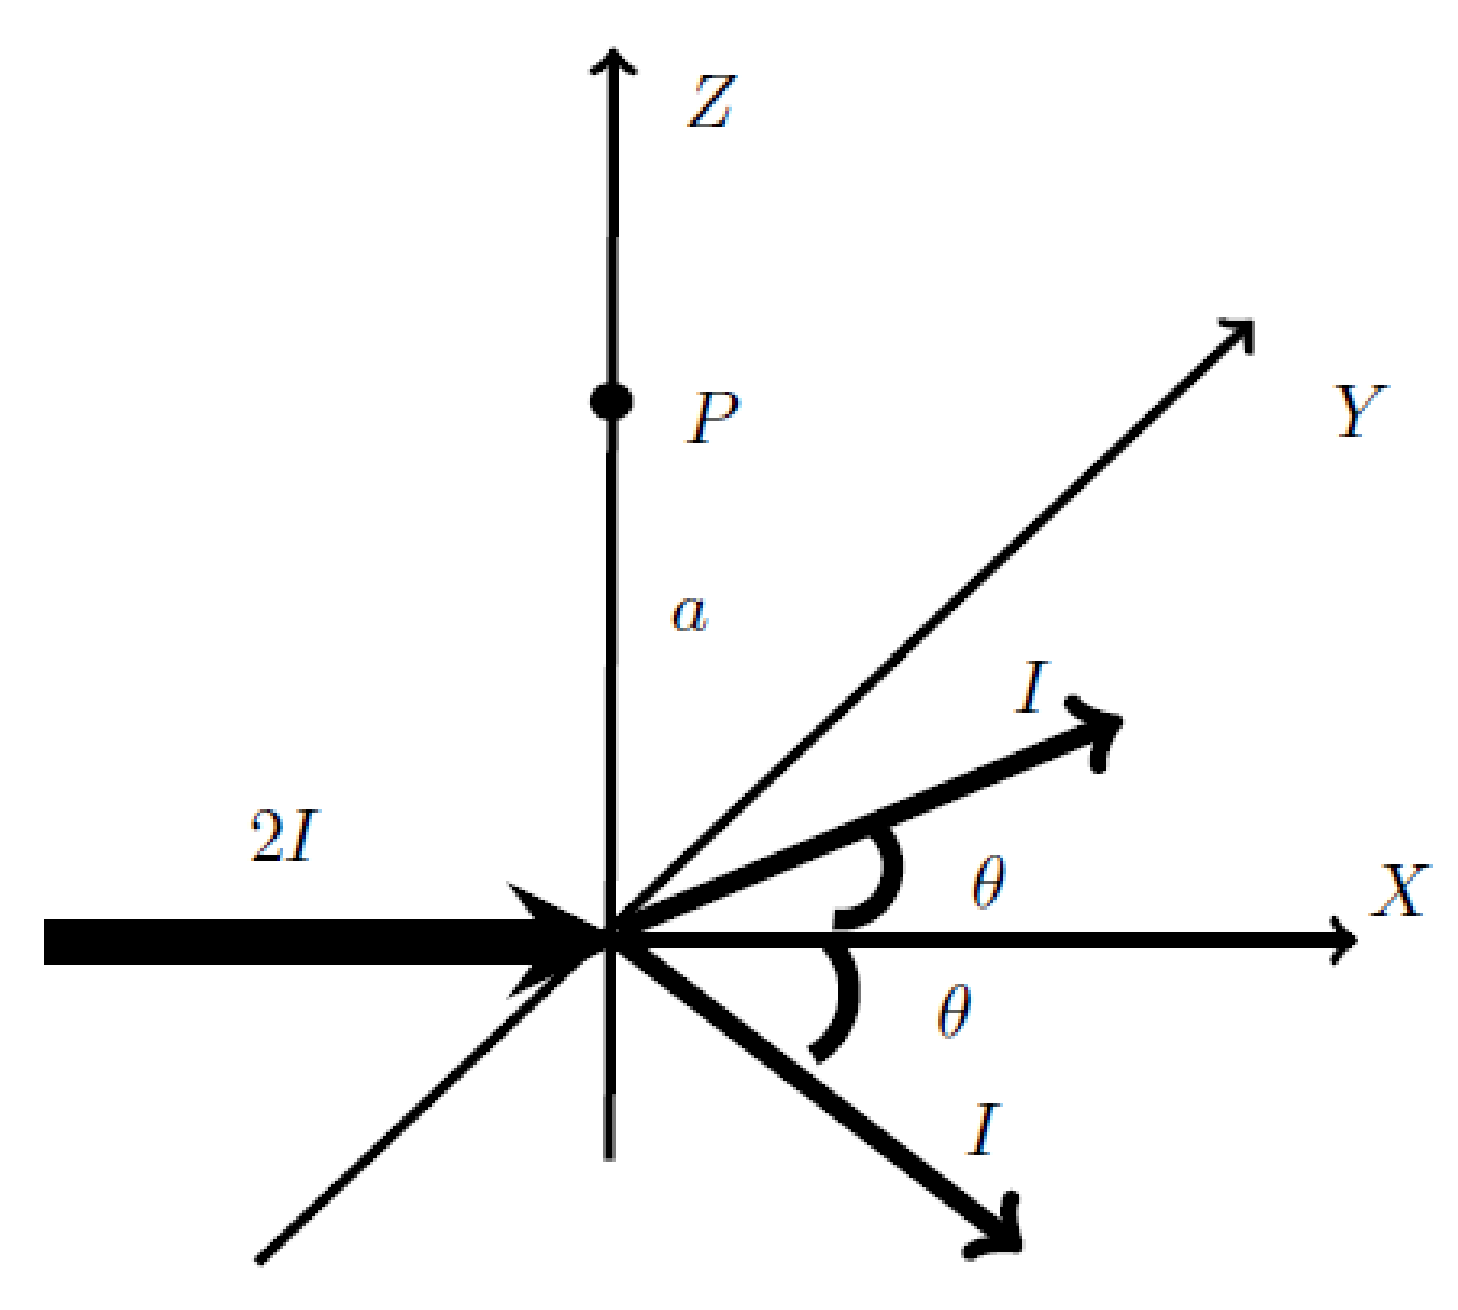
\includegraphics[width=5cm]{oz04/resources/oef-3-opgave.png}
    
%     \textbf{Figuur 4.3}
% \end{figure}

% \begin{description}[labelwidth=1.5cm, leftmargin=!]
%     \item[Geg. :]   Zie fig.;
% \end{description}

% % \begin{figure}[H]
% %     \centering
% %     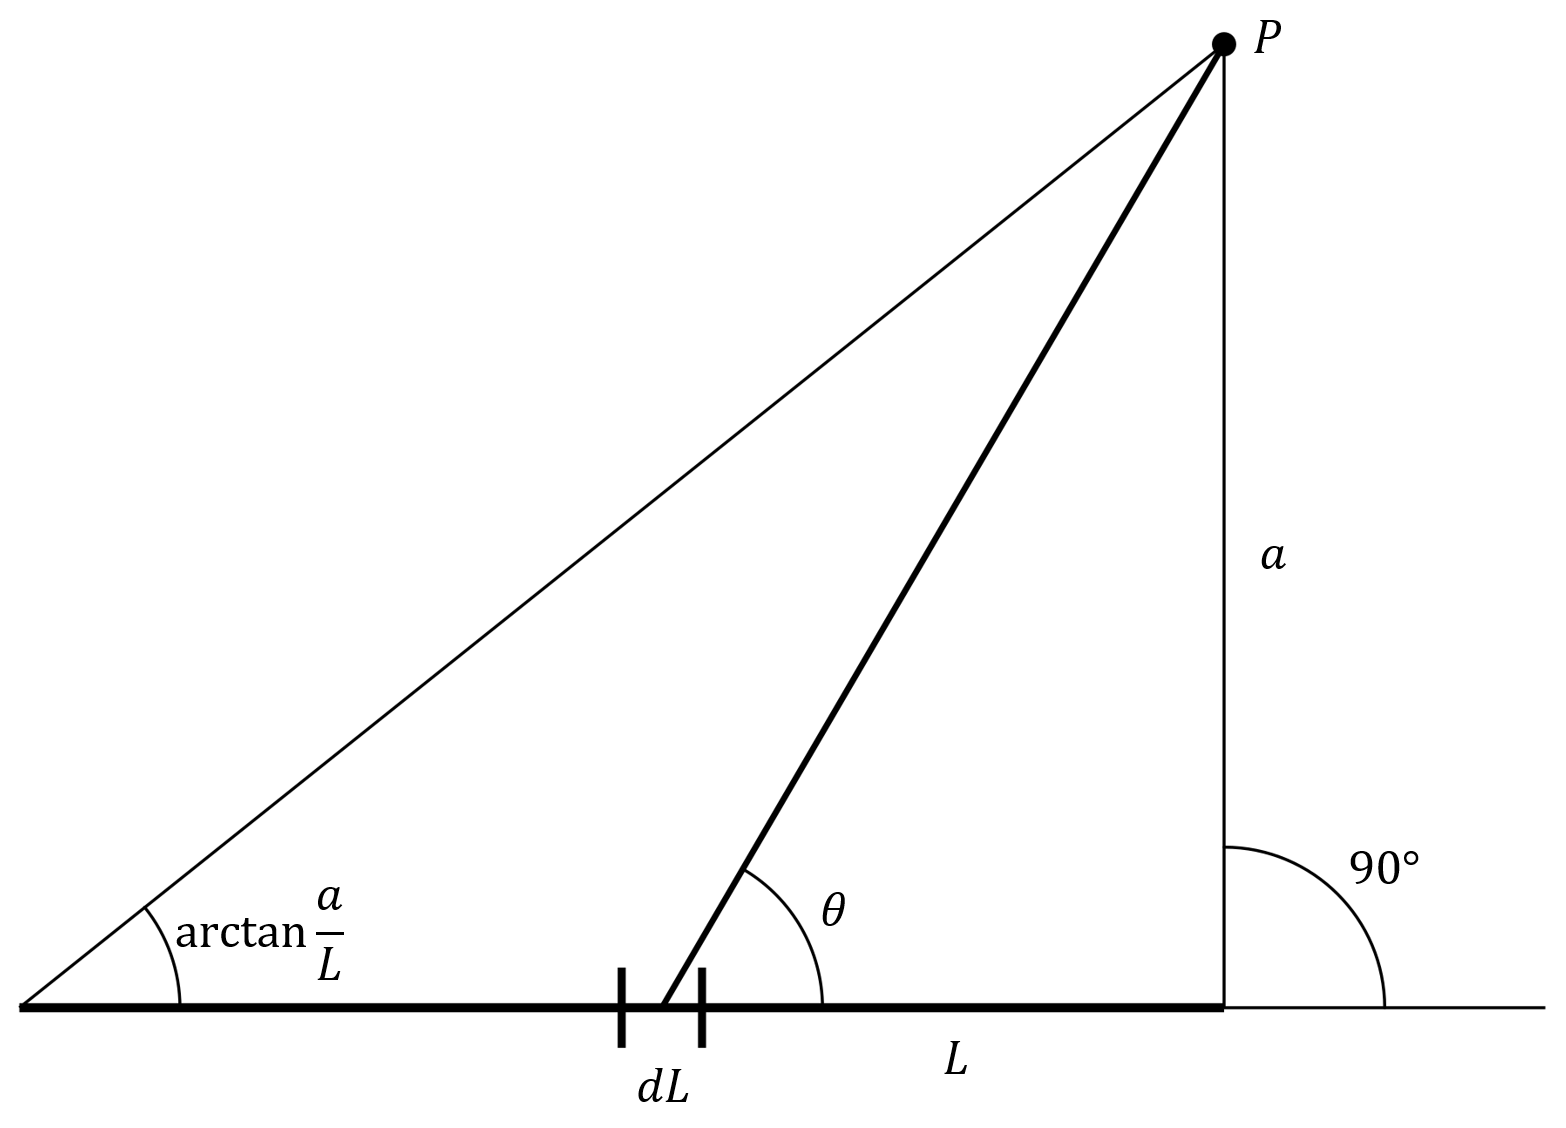
\includegraphics[width=7cm]{oz04/resources/oef-3-schets.png}
    
% %     \textbf{Schets 4.2}
% % \end{figure}

% \begin{description}[labelwidth=1.5cm, leftmargin=!]
%     \item[Gevr. :]  $ \vec{B}_y $;
%     \item[Opl. :] 

%     (Oplossing van Giancoli 4E Chapter 28 Problem 41)
    
%     The magnetic field at point $\mathrm{P}$ is found by integrating Eq. $28-5$ over the length of the current segment.
% $$
% \begin{aligned}
% \overrightarrow{\mathbf{B}} & =\int \frac{\mu_0 I}{4 \pi} \frac{d \vec{\ell} \times \hat{r}}{r^2}=\int \frac{\mu_0 I}{4 \pi} \frac{d \vec{\ell} \times \overrightarrow{\mathbf{r}}}{r^3}=\frac{\mu_0 I}{4 \pi} \int_{-d}^0 \frac{d x \hat{\mathbf{i}} \times(-x \hat{\mathbf{i}}+y \hat{\mathbf{j}})}{\left(x^2+y^2\right)^{3 / 2}}=\frac{\mu_0 I y}{4 \pi} \hat{\mathbf{k}} \int_{-d}^0 \frac{d x}{\left(x^2+y^2\right)^{3 / 2}} \\
% & =\left.\frac{\mu_0 I y}{4 \pi} \hat{\mathbf{k}} \frac{x}{y^2\left(x^2+y^2\right)^{1 / 2}}\right|_{-d} ^0=\frac{\mu_0 I}{4 \pi y} \frac{d}{\left(y^2+d^2\right)^{1 / 2}} \hat{\mathbf{k}}
% \end{aligned}
% $$
                    
                    
% \end{description}

% \vspace{1cm}